%% bare_conf.tex
%% V1.3
%% 2007/01/11
%% by Michael Shell
%% See:
%% http://www.michaelshell.org/
%% for current contact information.
%%
%% This is a skeleton file demonstrating the use of IEEEtran.cls
%% (requires IEEEtran.cls version 1.7 or later) with an IEEE conference paper.
%%
%% Support sites:
%% http://www.michaelshell.org/tex/ieeetran/
%% http://www.ctan.org/tex-archive/macros/latex/contrib/IEEEtran/
%% and
%% http://www.ieee.org/

%%*************************************************************************
%% Legal Notice:
%% This code is offered as-is without any warranty either expressed or
%% implied; without even the implied warranty of MERCHANTABILITY or
%% FITNESS FOR A PARTICULAR PURPOSE! 
%% User assumes all risk.
%% In no event shall IEEE or any contributor to this code be liable for
%% any damages or losses, including, but not limited to, incidental,
%% consequential, or any other damages, resulting from the use or misuse
%% of any information contained here.
%%
%% All comments are the opinions of their respective authors and are not
%% necessarily endorsed by the IEEE.
%%
%% This work is distributed under the LaTeX Project Public License (LPPL)
%% ( http://www.latex-project.org/ ) version 1.3, and may be freely used,
%% distributed and modified. A copy of the LPPL, version 1.3, is included
%% in the base LaTeX documentation of all distributions of LaTeX released
%% 2003/12/01 or later.
%% Retain all contribution notices and credits.
%% ** Modified files should be clearly indicated as such, including  **
%% ** renaming them and changing author support contact information. **
%%
%% File list of work: IEEEtran.cls, IEEEtran_HOWTO.pdf, bare_adv.tex,
%%                    bare_conf.tex, bare_jrnl.tex, bare_jrnl_compsoc.tex
%%*************************************************************************

% *** Authors should verify (and, if needed, correct) their LaTeX system  ***
% *** with the testflow diagnostic prior to trusting their LaTeX platform ***
% *** with production work. IEEE's font choices can trigger bugs that do  ***
% *** not appear when using other class files.                            ***
% The testflow support page is at:
% http://www.michaelshell.org/tex/testflow/



% Note that the a4paper option is mainly intended so that authors in
% countries using A4 can easily print to A4 and see how their papers will
% look in print - the typesetting of the document will not typically be
% affected with changes in paper size (but the bottom and side margins will).
% Use the testflow package mentioned above to verify correct handling of
% both paper sizes by the user's LaTeX system.
%
% Also note that the "draftcls" or "draftclsnofoot", not "draft", option
% should be used if it is desired that the figures are to be displayed in
% draft mode.
%
\documentclass[10pt,final,journal,a4paper]{IEEEtran}
% Add the compsoc option for Computer Society conferences.
%
% If IEEEtran.cls has not been installed into the LaTeX system files,
% manually specify the path to it like:
% \documentclass[conference]{../sty/IEEEtran}





% Some very useful LaTeX packages include:
% (uncomment the ones you want to load)


% *** MISC UTILITY PACKAGES ***
%
%\usepackage{ifpdf}
% Heiko Oberdiek's ifpdf.sty is very useful if you need conditional
% compilation based on whether the output is pdf or dvi.
% usage:
% \ifpdf
%   % pdf code
% \else
%   % dvi code
% \fi
% The latest version of ifpdf.sty can be obtained from:
% http://www.ctan.org/tex-archive/macros/latex/contrib/oberdiek/
% Also, note that IEEEtran.cls V1.7 and later provides a builtin
% \ifCLASSINFOpdf conditional that works the same way.
% When switching from latex to pdflatex and vice-versa, the compiler may
% have to be run twice to clear warning/error messages.






% *** CITATION PACKAGES ***
%
\usepackage{cite}
% cite.sty was written by Donald Arseneau
% V1.6 and later of IEEEtran pre-defines the format of the cite.sty package
% \cite{} output to follow that of IEEE. Loading the cite package will
% result in citation numbers being automatically sorted and properly
% "compressed/ranged". e.g., [1], [9], [2], [7], [5], [6] without using
% cite.sty will become [1], [2], [5]--[7], [9] using cite.sty. cite.sty's
% \cite will automatically add leading space, if needed. Use cite.sty's
% noadjust option (cite.sty V3.8 and later) if you want to turn this off.
% cite.sty is already installed on most LaTeX systems. Be sure and use
% version 4.0 (2003-05-27) and later if using hyperref.sty. cite.sty does
% not currently provide for hyperlinked citations.
% The latest version can be obtained at:
% http://www.ctan.org/tex-archive/macros/latex/contrib/cite/
% The documentation is contained in the cite.sty file itself.






% *** GRAPHICS RELATED PACKAGES ***
%
\ifCLASSINFOpdf
  % \usepackage[pdftex]{graphicx}
  % declare the path(s) where your graphic files are
  % \graphicspath{{../pdf/}{../jpeg/}}
  % and their extensions so you won't have to specify these with
  % every instance of \includegraphics
  % \DeclareGraphicsExtensions{.pdf,.jpeg,.png}
\else
  % or other class option (dvipsone, dvipdf, if not using dvips). graphicx
  % will default to the driver specified in the system graphics.cfg if no
  % driver is specified.
  % \usepackage[dvips]{graphicx}
  % declare the path(s) where your graphic files are
  % \graphicspath{{../eps/}}
  % and their extensions so you won't have to specify these with
  % every instance of \includegraphics
  % \DeclareGraphicsExtensions{.eps}
\fi
% graphicx was written by David Carlisle and Sebastian Rahtz. It is
% required if you want graphics, photos, etc. graphicx.sty is already
% installed on most LaTeX systems. The latest version and documentation can
% be obtained at: 
% http://www.ctan.org/tex-archive/macros/latex/required/graphics/
% Another good source of documentation is "Using Imported Graphics in
% LaTeX2e" by Keith Reckdahl which can be found as epslatex.ps or
% epslatex.pdf at: http://www.ctan.org/tex-archive/info/
%
% latex, and pdflatex in dvi mode, support graphics in encapsulated
% postscript (.eps) format. pdflatex in pdf mode supports graphics
% in .pdf, .jpeg, .png and .mps (metapost) formats. Users should ensure
% that all non-photo figures use a vector format (.eps, .pdf, .mps) and
% not a bitmapped formats (.jpeg, .png). IEEE frowns on bitmapped formats
% which can result in "jaggedy"/blurry rendering of lines and letters as
% well as large increases in file sizes.
%
% You can find documentation about the pdfTeX application at:
% http://www.tug.org/applications/pdftex





% *** MATH PACKAGES ***
%
\usepackage[cmex10]{amsmath}
% A popular package from the American Mathematical Society that provides
% many useful and powerful commands for dealing with mathematics. If using
% it, be sure to load this package with the cmex10 option to ensure that
% only type 1 fonts will utilized at all point sizes. Without this option,
% it is possible that some math symbols, particularly those within
% footnotes, will be rendered in bitmap form which will result in a
% document that can not be IEEE Xplore compliant!
%
% Also, note that the amsmath package sets \interdisplaylinepenalty to 10000
% thus preventing page breaks from occurring within multiline equations. Use:
%\interdisplaylinepenalty=2500
% after loading amsmath to restore such page breaks as IEEEtran.cls normally
% does. amsmath.sty is already installed on most LaTeX systems. The latest
% version and documentation can be obtained at:
% http://www.ctan.org/tex-archive/macros/latex/required/amslatex/math/





% *** SPECIALIZED LIST PACKAGES ***
%
%\usepackage{algorithmic}
\usepackage{algorithm}

% algorithmic.sty was written by Peter Williams and Rogerio Brito.
% This package provides an algorithmic environment fo describing algorithms.
% You can use the algorithmic environment in-text or within a figure
% environment to provide for a floating algorithm. Do NOT use the algorithm
% floating environment provided by algorithm.sty (by the same authors) or
% algorithm2e.sty (by Christophe Fiorio) as IEEE does not use dedicated
% algorithm float types and packages that provide these will not provide
% correct IEEE style captions. The latest version and documentation of
% algorithmic.sty can be obtained at:
% http://www.ctan.org/tex-archive/macros/latex/contrib/algorithms/
% There is also a support site at:
% http://algorithms.berlios.de/index.html
% Also of interest may be the (relatively newer and more customizable)
% algorithmicx.sty package by Szasz Janos:
% http://www.ctan.org/tex-archive/macros/latex/contrib/algorithmicx/




% *** ALIGNMENT PACKAGES ***
%
\usepackage{array}
% Frank Mittelbach's and David Carlisle's array.sty patches and improves
% the standard LaTeX2e array and tabular environments to provide better
% appearance and additional user controls. As the default LaTeX2e table
% generation code is lacking to the point of almost being broken with
% respect to the quality of the end results, all users are strongly
% advised to use an enhanced (at the very least that provided by array.sty)
% set of table tools. array.sty is already installed on most systems. The
% latest version and documentation can be obtained at:
% http://www.ctan.org/tex-archive/macros/latex/required/tools/


\usepackage{mdwmath}
\usepackage{mdwtab}
% Also highly recommended is Mark Wooding's extremely powerful MDW tools,
% especially mdwmath.sty and mdwtab.sty which are used to format equations
% and tables, respectively. The MDWtools set is already installed on most
% LaTeX systems. The lastest version and documentation is available at:
% http://www.ctan.org/tex-archive/macros/latex/contrib/mdwtools/


% IEEEtran contains the IEEEeqnarray family of commands that can be used to
% generate multiline equations as well as matrices, tables, etc., of high
% quality.


\usepackage{eqparbox}
% Also of notable interest is Scott Pakin's eqparbox package for creating
% (automatically sized) equal width boxes - aka "natural width parboxes".
% Available at:
% http://www.ctan.org/tex-archive/macros/latex/contrib/eqparbox/





% *** SUBFIGURE PACKAGES ***
%\usepackage[tight,footnotesize]{subfigure}
% subfigure.sty was written by Steven Douglas Cochran. This package makes it
% easy to put subfigures in your figures. e.g., "Figure 1a and 1b". For IEEE
% work, it is a good idea to load it with the tight package option to reduce
% the amount of white space around the subfigures. subfigure.sty is already
% installed on most LaTeX systems. The latest version and documentation can
% be obtained at:
% http://www.ctan.org/tex-archive/obsolete/macros/latex/contrib/subfigure/
% subfigure.sty has been superceeded by subfig.sty.



%\usepackage[caption=false]{caption}
%\usepackage{caption}
%\usepackage[font=footnotesize, captions=false]{subfig}
% subfig.sty, also written by Steven Douglas Cochran, is the modern
% replacement for subfigure.sty. However, subfig.sty requires and
% automatically loads Axel Sommerfeldt's caption.sty which will override
% IEEEtran.cls handling of captions and this will result in nonIEEE style
% figure/table captions. To prevent this problem, be sure and preload
% caption.sty with its "caption=false" package option. This is will preserve
% IEEEtran.cls handing of captions. Version 1.3 (2005/06/28) and later 
% (recommended due to many improvements over 1.2) of subfig.sty supports
% the caption=false option directly:
%\usepackage[caption=false,font=footnotesize]{subfig}
%
% The latest version and documentation can be obtained at:
% http://www.ctan.org/tex-archive/macros/latex/contrib/subfig/
% The latest version and documentation of caption.sty can be obtained at:
% http://www.ctan.org/tex-archive/macros/latex/contrib/caption/




% *** FLOAT PACKAGES ***
%
\usepackage{fixltx2e}
% fixltx2e, the successor to the earlier fix2col.sty, was written by
% Frank Mittelbach and David Carlisle. This package corrects a few problems
% in the LaTeX2e kernel, the most notable of which is that in current
% LaTeX2e releases, the ordering of single and double column floats is not
% guaranteed to be preserved. Thus, an unpatched LaTeX2e can allow a
% single column figure to be placed prior to an earlier double column
% figure. The latest version and documentation can be found at:
% http://www.ctan.org/tex-archive/macros/latex/base/



%\usepackage{stfloats}
% stfloats.sty was written by Sigitas Tolusis. This package gives LaTeX2e
% the ability to do double column floats at the bottom of the page as well
% as the top. (e.g., "\begin{figure*}[!b]" is not normally possible in
% LaTeX2e). It also provides a command:
%\fnbelowfloat
% to enable the placement of footnotes below bottom floats (the standard
% LaTeX2e kernel puts them above bottom floats). This is an invasive package
% which rewrites many portions of the LaTeX2e float routines. It may not work
% with other packages that modify the LaTeX2e float routines. The latest
% version and documentation can be obtained at:
% http://www.ctan.org/tex-archive/macros/latex/contrib/sttools/
% Documentation is contained in the stfloats.sty comments as well as in the
% presfull.pdf file. Do not use the stfloats baselinefloat ability as IEEE
% does not allow \baselineskip to stretch. Authors submitting work to the
% IEEE should note that IEEE rarely uses double column equations and
% that authors should try to avoid such use. Do not be tempted to use the
% cuted.sty or midfloat.sty packages (also by Sigitas Tolusis) as IEEE does
% not format its papers in such ways.





% *** PDF, URL AND HYPERLINK PACKAGES ***
%
\usepackage{url}
% url.sty was written by Donald Arseneau. It provides better support for
% handling and breaking URLs. url.sty is already installed on most LaTeX
% systems. The latest version can be obtained at:
% http://www.ctan.org/tex-archive/macros/latex/contrib/misc/
% Read the url.sty source comments for usage information. Basically,
% \url{my_url_here}.

\usepackage{epsfig}
\usepackage{graphicx}
%\usepackage{subfloat}
%\usepackage{subcaption}
\usepackage[T1]{fontenc}
\usepackage{mwe}
\usepackage{subfig}
\usepackage{float}
\usepackage{algcompatible}

%\usepackage{algpseudocode}
%\usepackage{algpseudocode}
%\usepackage{subfloat}
%\usepackage[section]{placeins}

% *** Do not adjust lengths that control margins, column widths, etc. ***
% *** Do not use packages that alter fonts (such as pslatex).         ***
% There should be no need to do such things with IEEEtran.cls V1.6 and later.
% (Unless specifically asked to do so by the journal or conference you plan
% to submit to, of course. )


% correct bad hyphenation here
\hyphenation{op-tical net-works semi-conduc-tor}


\begin{document}
%
% paper title
% can use linebreaks \\ within to get better formatting as desired
\title{Peer-Assisted Content Distribution Aided by Video Popularity Evolution Model}

\author{\IEEEauthorblockN{Mohamad Dikshie Fauzie\IEEEauthorrefmark{1} \quad
Achmad Husni Thamrin\IEEEauthorrefmark{1} \quad
Jun Murai\IEEEauthorrefmark{2}}
\IEEEauthorblockA{\IEEEauthorrefmark{1}Graduate School of Media and Governance} \quad
\IEEEauthorblockA{\IEEEauthorrefmark{2}Faculty of Environment and Information Studies\\ 
Keio University, 252-0882 Kanagawa, Japan \\
dikshie@sfc.wide.ad.jp \quad\quad husni@ai3.net \quad\quad jun@wide.ad.jp}
}




% use for special paper notices
%\IEEEspecialpapernotice{(Invited Paper)}




% make the title area
\maketitle


\begin{abstract}
%\boldmath
%Content distribution network (CDN) is widely used to efficiently deliver streaming media. 
%The CDN with dedicated network bandwidths and hardware supports can provide high-quality streaming services but at a high cost. 
%On the other side, the rise of peer-to-peer (P2P) networks are scalable but do not guarantee high quality streaming service due to the transient nature of peers.
In this paper, we present peer-assisted CDN model, the peer-to-peer networks that can be used to help CDN to deliver streaming media.
Our peer-assisted CDN model is aided by Youtube VoD views popularity model called CPPro.
We have comparatively evaluated CPPro through trace-driven simulations with synthetic workloads.
We use three scenarios in our simulation which are 
(a) the video popularity in the CPPro system follows the global popularity of the video.
(b) the video popularity in the CPPro system is lagged behind the global popularity by several weeks.
(c) the video popularity in the CPPro is unrelated to the global popularity.
Our results show that CPPro gives lower number of replicas while maintaining same number of peers contribution compare to counterpart work. 
We also do the significance to the number of replicas using the Kolmogorov-Smirnov statistic on two samples and we find our results are significant ($p-values < 0.1$). 

\end{abstract}
% IEEEtran.cls defaults to using nonbold math in the Abstract.
% This preserves the distinction between vectors and scalars. However,
% if the conference you are submitting to favors bold math in the abstract,
% then you can use LaTeX's standard command \boldmath at the very start
% of the abstract to achieve this. Many IEEE journals/conferences frown on
% math in the abstract anyway.

% no keywords
\begin{IEEEkeywords}
Internet Video on Demand (VoD), P2P, CDN, and Caching.
\end{IEEEkeywords}

% For peer review papers, you can put extra information on the cover
% page as needed:
% \ifCLASSOPTIONpeerreview
% \begin{center} \bfseries EDICS Category: 3-BBND \end{center}
% \fi
% For peerreview papers, this IEEEtran command inserts a page break and
% creates the second title. It will be ignored for other modes.
%\IEEEpeerreviewmaketitle


\section{Introduction}
Streaming content, especially video, represents a significant fraction of the traffic volume on the Internet, and it has become a standard practice to deliver this type of content using Content Delivery Networks (CDNs) such as Akamai and Limelight for better scaling and quality of experience for the end users. 
For example, YouTube uses Google cache and MTV uses Akamai in their operations.

With the spread of broadband Internet access at a reasonable flat monthly rate, users are connected to the Internet 24 hours a day and they can download and share multimedia content. P2P (peer to peer) applications are also widely deployed. 
In China, P2P is very popular; we see many P2P applications from China such as PPLive, PPStream, UUSe, Xunlei, etc. \cite{Vu:2010:UOC:1865106.1865115}. 
Some news broadcasters also rely on P2P technology to deliver popular live events. 
For example, CNN uses the Octoshape \cite{octoshape} solution that enables their broadcast to scale and offer good video quality as the number of users increases.

From the Internet provider point of view, the presence of so many always-on users suggests that it is possible to delegate a portion of computing, storage and networking tasks to the users, thus creating P2P networks where users can share files and multimedia content. 
Starting from file sharing protocols, P2P architectures have evolved toward video on demand and support for live events.

%A P2P based architecture usually requires a sufficient number of nodes supplying the data (seeders) to start the distribution process among the joining peers.  
%A peer usually offers a low outbound streaming rate due to the traditional asymmetrical DSL home connectivity and hence multiple peers must jointly stream contents to a requesting peer (leecher).  
%The decentralized, uncoordinated operation implies that scaling to a high number of peers comes with side effects.  
%Typical problems of a P2P streaming architecture are low stream quality with undesirable disruptions, resource unfairness due to heterogeneous peer resources, and high startup delay.  
%Moreover, current P2P applications are not aware of the underlying network and may conflict with the ISP routing policies and business model.

%A number of P2P streaming applications have been designed, analyzed and deployed, attracting a significant number of users.  
%Research studies and deployment experiences have both demonstrated that P2P is a promising solution in terms of scalability and deployment costs.  
%On the other hand, the heterogeneous nature and unstable behavior of the peers contributing bandwidth and computational resources, along with the networking issues, affect the user experience and limit the commercial success of P2P video streaming applications.
Alternatively, video contents can be efficiently distributed on services offered by managed network architectures and CDN companies.
The major issues of CDN are high deployment cost and good but not unlimited scalability in the long term.  
Given the complementary features of P2P and CDN, in recent years some hybrid solutions have been proposed and applied to the operational of CDN \cite{Huang:2008:UHC:1496046.1496064,4772628,Yin:2009:DDH:1631272.1631279} to take the best of both approaches.
In Peer assisted CDN, users can download content from CDN nodes from or other users or peers. 
A user may cache the content after download to serve requests from other users. 
Due to the complexity of the behavior of peers, the process should be done in the home gateway user where the ISP can control it.

In this work, we will revisit Guo et al.'s, \cite{1613869} PROP as a basis to evaluate peer-assisted CDN and propose an improvement to the model for the PROP called CPPro.
This system is called CPPro abbreviated from out technical term "CDN-P2P Project".
We will take Youtube as an example of an Internet VoD service model.
In the Youtube service model, we can get data such as (1) the time when a video is uploaded and (2) number of access or number of view.
We can get such data using Youtube's API.
In seminal work, Borghol et al., \cite{Borghol:2011:CMP:2039452.2039717} used the above information to estimate when a video will become very popular.
They divide a video's popularity into three phases: before-peak phase, at-peak phase, and after-peak phase.
We will use an estimate of a video's popularity phases for helping PROP.
We will explain video popularity in Sec.\ref{popularity}.
Our contribution is as follows:
(1) We use the idea of VoD view popularity model to aid the PROP model. 
To the best of our knowledge, the combination of the PROP model and the VoD view popularity model is new.
(2) From simulation-based experiments, we find that peer contributions in CPPro are almost as good as  PROP while the numbers of replicas are lower than PROP resulting in a reduction of resources required.

Our paper presentation as follows: (1) we describe related work in sect.\ref{relatedwork}; (2) we explain detail of Youtube popularity evolution model in sect.\ref{popularity}; (3) we explain the caching strategy for CDN and peer in sect.\ref{systemdescription}; (4) we explain our simulation design, simulator, and its evaluation in sect.\ref{evaluation}.
Finally, we present our conclusions in section \ref{conclusion}.

\section{Related Work}\label{relatedwork}
Content Distribution Networks with peer assist have been successfully deployed on the Internet, such as Akamai \cite{Zhao:2013:PCD:2504730.2504752}, \cite{Huang:2008:UHC:1496046.1496064} and LiveSky \cite{Yin:2010:LEC:1823746.1823750}.  
The authors of \cite{Zhao:2013:PCD:2504730.2504752} examine the risks and benefits of peer-assisted content distribution in Akamai and measure the effectiveness of its peer-assisted approach. 
The authors of \cite{Huang:2008:UHC:1496046.1496064} conclude from two real world traces that hybrid CDN-P2P can significantly reduce the cost of content distribution and can scale to cope with the exponential growth of Internet video content.  
Yin et al. \cite{Yin:2010:LEC:1823746.1823750} described commercial operation of a peer-assisted CDN in China.  
LiveSky solved several challenges in the system design, such as dynamic resource scaling of P2P, low startup latency, ease of P2P integration with the existing CDN infrastructure, and network friendliness and upload fairness in the P2P operation.  
Xu et al.\cite{DBLP:journals/corr/abs-1212-4915} used game-theory to show the right cooperative profit distribution of P2P can help the ISP to maximize the utility.  
Their model can easily be implemented in the context of current Internet economic settlements.  
Misra et al.\cite{Misra:2010:IPS:1811099.1811064} also mentioned the importance of P2P architecture to support content delivery networks.
The authors use cooperative game theory to formulate simple compensation rules for users who run P2P to support content delivery networks.

The idea of telco- or ISP-managed CDN has been proposed in recent years.  
The complexity of the CDN business encourages telcos and ISPs to manage their own CDN, rather than allow others to run CDNs on their networks.  
It has been shown that it is cost effective \cite{federation}\cite{norton2011internet}. 
Kamiyama et al. \cite{NoriakiKAMIYAMA2013} proposed optimally ISP operated CDN.
Kamiyama et al. mentioned that, in order to deliver large and rich Internet content to users, ISPs need to put their CDNs in data centers.  
The locations are limited while the storage is large, making this solution effective; using optimum placement algorithm based on real ISP network topologies.  
The authors found that inserting a CDN into an ISP's ladder-type network is effective in reducing the hop count, thus reduce total link cost.  
Based on the author definition: Ladder-type network is a network with a maximum degree under $10$.
Cisco has initiated an effort to connect telco- or ISP-managed CDNs to each other, to form a CDN federation \cite{federation} using open standards \cite{cdni}.  
They argue that the current CDN architecture is not close enough to the users and ISPs can fill this position.

The idea of utilizing the user's computation power to support ISP operation is not new.  
The Figaro project \cite{figaro} proposed the residential gateway as an integrator of different networks and services, becoming an Internet-wide distributed content management for a proposed future Internet architecture \cite{figaro}.  
Cha et al.,\cite{Cha:2008:NTP:1855641.1855646} performed trace analysis and found that an IPTV architecture powered by P2P can handle a much larger number of channels, with lower demand for infrastructure compared to IP multicast.  
Jiang et al. \cite{Jiang:2012:OMD:2413176.2413193} proposed scalable and adaptive content replication and request routing for CDN servers located in users' home gateways.  
Maki et al.,\cite{NaoyaMAKI2012} propose traffic engineering for peer-assisted CDN to control the behavior of clients, and present a solution for optimizing the selection of content files.
Mathieu et al., \cite{6249305} are using data gathered from France telecom network to calculate reduction of network load if customers are employed as peer-assisted content delivery.

Guo et al., \cite{1613869} work's PROP is closest with our work.
%because we use that work as comparison and we use author's utility function.
PROP uses local system (local counter) to calculate the segment popularity in peer-assisted proxy system. 
PROP uses popularity for proxy cache replacement strategy. 
In peer side, the author use utility function for cache replacement strategy.
A utility function assigns numerical value to outcomes, in such a way that outcomes with higher utility are always preferred of outcomes with lower utilities.
In PROP's utility function, the difference between very popular videos and unpopular video is very difficult to differentiate. 
The utility function is also function from popularity.
While the authors successfully show that the results are very good, the peer-assisted system behavior over time is not explain because the author focus on properties such as proxy cache size variations and peer cache size variations.
The explanation of the optimal number of replicas is not also clear because unavailable information when the snapshot is taken.  
In our work, we complement Guo et al., \cite{1613869} work with VoD viewing popularity evolution model and describe the behavior of the peer-assisted CDN over the time.

\begin{figure}[!t]
\begin{center}
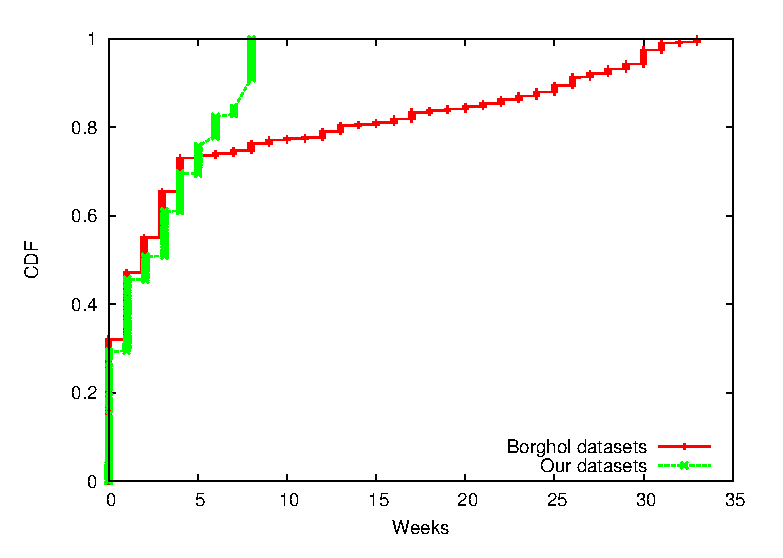
\includegraphics[scale=0.6]{graphs/timetopeak.eps}
\end{center}
\caption{Time to peak empirical distribution data from \cite{Borghol:2011:CMP:2039452.2039717}.}
\label{fig:timetopeak}
\end{figure} 


\begin{figure}[!t]
\begin{center}
\includegraphics[scale=0.6]{graphs/datadistribution.eps}
\end{center}
\caption{View rate distribution versus week relative to at-peak phase week for every video, where y-axis in log scale.
Every point lies in negative x-axis mean view rate of every video in before-peak phase.
Every point lies in x-axis$=0$ mean view rate of every video at-peak phase. 
Every point lies in positive x-axis mean view rate of every video in after-peak phase.
As we see in this graph, while fig.\ref{fig:timetopeak} mentioned that $75\%$ of videos reach at-peak within six weeks, we also see that some vides reach at-peak after six weeks.
Data from \cite{Borghol:2011:CMP:2039452.2039717}. }
\label{fig:viewratedistribution}
\end{figure} 

% \begin{figure*}[!t]
% \centering
% \subfloat[Transformation of view rate distribution. We add week number and make it as $x$-axis, View rate as $y$-axis, and relative week to peak as $z$-axis. \label{fig:viewratedistexample}] {
% 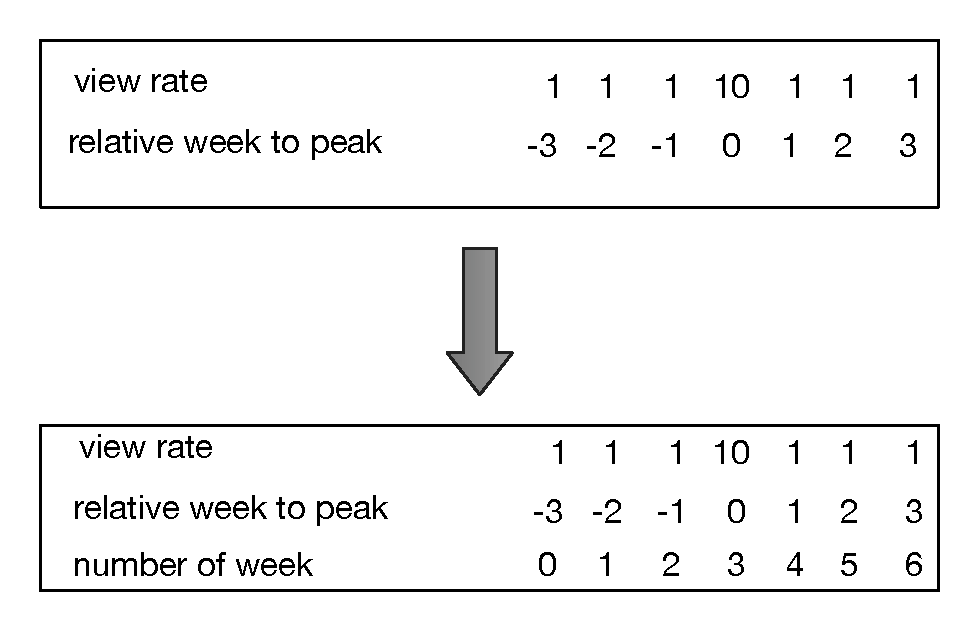
\includegraphics[width=7cm]{graphs/transformasi.eps} 
% }
% \hfill
% \subfloat[2D visualization of view rate distribution after transformation where $x$-axis is week number, $y$-axis is view rate. 
% Popularity phase of a requested video denote by circle can be determine by averaging relative week to peak values from the nearest points which are A and B.
% \label{fig:viewratedistexamplered}] {
% \includegraphics[width=7cm]{graphs/transformasi3.eps} 
% }
% \caption{Transformation of view rate distribution dataset and 2D visualization of view rate distribution from fig.~\ref{fig:viewratedistexamplered}. X-axis is week number and Y-axis is view rate.
% }
% \label{fig:transformand2d}
% \end{figure*}


\section{Determining Internet VoD Popularity Phase}\label{popularity}

The objective of determining the Internet VoD popularity phase is to determine whether a video is at before-peak, at-peak, or after-peak phase, to be used by peers in their caching strategy.
For this purpose we use the Youtube content popularity dataset from Borghol et. al.,\cite{Borghol:2011:CMP:2039452.2039717}  which contains the data of 29791 videos, including the view count and upload time, during 36 weeks of measurements.
Figure~\ref{fig:timetopeak} is cummulative distribution function (CDF) the time-to-peak distribution from Borghol et. al.,\cite{Borghol:2011:CMP:2039452.2039717}  which shows that around three-quarters of the videos peak within the first six weeks after upload.
The time-to-peak is exponentially distributed up-to the sixth week, and it is uniform beyond the sixth week.
Borghol et al., \cite{Borghol:2011:CMP:2039452.2039717} define time-to-peak for a video as its age (time since upload) at which its weekly viewing rate is the highest during measurement (from the first week until end of measurement).
Because we know the peak time (at-peak phase) of every video, we can also find the before-peak phase and after-phase of every video. 
For detail we refer the readers to \cite{Borghol:2011:CMP:2039452.2039717}.

Suppose a video $v$ in Borghol dataset has a viewing rate $r_v(t)$, $0 <= t < t_f$, and $r_v(t)$ peaks at $t_{vp}$.
The data is transformed by including the relative time-to-peak, such that each data point is a 2-tuple: video rate and relative time to peak, i.e., $rp_v(t) = ( r_v(t), tp(t) ), tp(t) = t - t_{vp}$.
Figure~\ref{fig:viewratedistribution} shows the Borghol's dataset with time axis for each video is translated by $t_{vp}$ to the left, such that each video peaks at time $0$.
%The algorithm to shift the week of the at-peak phase to zero for every video in dataset is shown as pseudo code in \ref{alg1}.

%%%% tandai %%%%%%
% \begin{algorithm}
% \caption{Shifting relative week to at-peak for every video in dataset}
% \label{alg1}
% \begin{algorithmic}[1]
% \REQUIRE $data \leftarrow view rate$

% \STATE length $\leftarrow$ 36 \COMMENT{number of weeks}
% \FOR{every video}
% \STATE viewratemax $\leftarrow$ max(data) \COMMENT{find max view rate from a list}
% \STATE index $\leftarrow$ findindex(viewratemax)\COMMENT{find element index of maximum view rate}
% \FOR{$i=0$ to $length$ }
% \STATE $j[i]$ $\leftarrow$ $0$ \COMMENT{initialization with 0}
% \ENDFOR
% \FOR{$i=0$ to $length$}
% \STATE $j[i]$ $\leftarrow$ $(i-index)$ \COMMENT{we got relative week to at-peak}
% \ENDFOR
% \ENDFOR
% \end{algorithmic}
% \end{algorithm}
%%%%%%%%%%%%%%%%%

\begin{algorithm}
\caption{Averaging relative weeks from the nearest neighbor points}
\label{alg2}
\begin{algorithmic}[1]
\REQUIRE {dataset that consist of weeknumber, viewrate, and relative week to at peak.}

\STATE $t$ $\leftarrow$ read(weeknumber) \COMMENT{read week number from dataset}
\STATE $r_v$ $\leftarrow$ read(viewrate) \COMMENT{read view rate from dataset}
\STATE $tp$ $\leftarrow$ read(relativeweeksatpeak) \COMMENT{read relative week at peak from dataset}

%\COMMENT{a requested video has week number and view rate}
\STATE $t_e$ \COMMENT{week number of a requested video}
\STATE $r_e$ \COMMENT{view rate of a requested video}

\STATE $t_e^{before}$ $\leftarrow$ $(t_e - 1)$ \COMMENT{at one week before}
\STATE $tp_{before}$ $\leftarrow$ $find\_tp(t_e^{before},r_e,t,r_v,tp)$

\STATE $t_e^{at}$ $\leftarrow$ $(t_e)$ \COMMENT{at same week}
\STATE $tp_{at}$ $\leftarrow$ $find\_tp(t_e^{at},r_e,t,r_v,tp)$

\STATE $t_e^{after}$ $\leftarrow$ $(t_e+1)$ \COMMENT{at one week after}
\STATE $tp_{after}$ $\leftarrow$ $find\_tp(t_e^{after},r_e,t,r_v,tp)$

\STATE $tp\_final$ $\leftarrow$ $average(tp_{before}, tp_{at}, tp_{after})$
\IF{$tp\_final$ $<$ $0$}
\STATE $phase$ $\leftarrow$ $before$
\ELSIF{$tp\_final$ $==$ $0$}
\STATE $phase$ $\leftarrow$ $at$
\ELSE
\STATE $phase$ $\leftarrow$ $after$
\ENDIF
\end{algorithmic}
\end{algorithm}


% \begin{algorithm}
% \caption{Findnearestpoints function}
% \label{alg3}
% \begin{algorithmic}[1]
% \REQUIRE {xs, ysearch, x, y, z.}

% %\COMMENT{slice the dataset}
% \STATE $len_1$ $\leftarrow$ $length(xs)$
% \FOR{$i=0$ to $len_1$}
% \IF{$x[i]$ $==$ $xs$} 
% %\COMMENT{get data that only for x1}
% \STATE $tempx[i]$ $\leftarrow$ $x[i]$
% \STATE $tempy[i]$ $\leftarrow$ $y[i]$
% \STATE $tempz[i]$ $\leftarrow$ $z[i]$
% \ENDIF
% \ENDFOR

% \STATE $len_2 \leftarrow length(tempy[i])$
% \FOR{$i=0$ to $len_2$}
%     \IF{$tempy[i]$ $==$ $ysearch$}
%     \STATE $result[i]$ $\leftarrow$ $tempz[i]$ \COMMENT {get relative week only for ysearch}
%     \ENDIF
% \ENDFOR

% \STATE return(result)
% \end{algorithmic}
% \end{algorithm}



% \begin{algorithm}
% \caption{Determining popularity phase for the first time access}
% \label{alg4}
% \begin{algorithmic}[1]
% \REQUIRE{Sorted PDF of time to peak in the form of list of tuple [(prob,week number),$\cdots$] and $t$ which is week number of a requested video}

% \STATE $n$ $\leftarrow$ $36$ \COMMENT{number of measurement weeks}

% \IF{$t$ $>$ $36$}
% \STATE $phase$ $\leftarrow$ $after$
% \ELSE
% \STATE $result$ $\leftarrow$ $weightedsample(items,n)$
% \ENDIF

% \FOR{$i=0$ to $length(result)$}
% \STATE $temp[i]$ $\leftarrow$ $result[i])$ \COMMENT{add every element of result to a list temp}
% \ENDFOR
% \STATE $temp$ $\leftarrow$ $sorted(temp)$ \COMMENT{sort temp} 

% \STATE $total$ $\leftarrow$ $0$
% \FOR{$i=0$ to $t$}
% \STATE $numbercount$ $\leftarrow$ $count(temp,i)$ \COMMENT{count how many t's value inside temp}
% \STATE $total$ $\leftarrow$ $total$ $+$ $numbercount$ \COMMENT{add the number count to total}
% \ENDFOR
% \STATE $total$ $\leftarrow$ $total/36$ \COMMENT{divide total by total number of week from dataset}
% \IF{$total \le 0.5$}
% \STATE $phase$ $\leftarrow$ $before$
% \ELSIF{$total$ $>$ $0.5$ and $total$ $\le$ $0.75$}
% \STATE $phase$ $\leftarrow$ $at$ 
% \ELSE
% \STATE $phase$ $\leftarrow$ $after$ 
% \ENDIF

% \end{algorithmic}
% \end{algorithm}

% \begin{algorithm}
% \caption{Weighted sample (weighted probability sampling with replacement)}
% \label{alg5}
% \begin{algorithmic}[1]
% \REQUIRE {Sorted PDF of time to peak in the form of list of tuple [(prob,week number), $\cdots$]}

% \STATE $total$  $\leftarrow$ $1$
% \STATE $i$ $\leftarrow$ $0$ 
% \STATE $w$ $\leftarrow$ $items[0][0]$ \COMMENT{the smallest probability}
% \STATE $v$ $\leftarrow$ $items[0][1]$ \COMMENT{week number the pair of the smallest probability}

% \WHILE{$n$} 
% \STATE $x$ $\leftarrow$ $total * (1*random() ^ {(1.0/n)})$
% \STATE $total$ $\leftarrow$ $(total - x)$
% \WHILE{$x > w$}
% \STATE $x \leftarrow (x-w)$
% \STATE $i \leftarrow (i+1)$
% \STATE $w \leftarrow items[i][0]$
% \STATE $v \leftarrow items[i][1]$
% \ENDWHILE
% \STATE $w \leftarrow (w-x)$
% \STATE $b$ $\leftarrow$ $append(v$) \COMMENT{add v value to a list b}
% \STATE $n$ $\leftarrow$ $(n-1)$
% \STATE return $b$
% \ENDWHILE

% \end{algorithmic}
% \end{algorithm}


\begin{algorithm}
\caption{Determine phase for the first access a requested video}
\label{alg3}
\begin{algorithmic}[1]
\REQUIRE {$t_e$ and time-to-peak distribution}

\STATE $len$ $\leftarrow$ 35 
\FOR{$i=0$ to $len$}
\STATE draw integer random number between $0$ and $35$ respect to time-to-peak distribution: 
$d$ $\leftarrow$ $draw\_integer\_random\_number()$
\ENDFOR

\STATE {$total \leftarrow 0$}
\FOR{$i=0$ to $t_e$}
\STATE $total$ $\leftarrow$ $total$ + $count(d,i)$ \COMMENT{counting how many each integer random number and sum those}
\ENDFOR
\STATE{$estphase$ $\leftarrow$ $total/36$}
\IF{$estphase$ $>$ $0.75$}
\STATE {phase $\leftarrow$ after-peak}
\ELSIF{$estphase \leq 0.75$ and $estphase > 0.5$}
\STATE {phase $\leftarrow$ at-peak}
\ELSE
\STATE {phase $\leftarrow$ before-peak}
\ENDIF
\end{algorithmic}
\end{algorithm}

In determining the phase of a requested video $e$ with known age $t_e$ and view rate $r_e$ at $t_e$, we find the three $r_v$ data points whose rates are closest to $r_e$ at $t_e$, $(t_e - 1)$, and $(t_e + 1)$, and then average the $tp$ of the three data points.
The phase of the requested video $e$ is estimated to be before-peak, at-peak, or after-peak based on whether the average is negative, $0$, or positive.
The view rate $r_e$ of a video is calculated by substracting the view counts at the time of the current and the previous video requests.
The pseudo code for averaging the $tp$ is shown in algorithm \ref{alg2}.
%The view rate $r_e$  of a video is calculated using the view counts at the time of the current and the previous video requests.
But when a video is being requested for the first time, the phase can only be estimated using the age of the video.
In this case, we draw 36 random integer numbers $s_i$, $0 <= i <= 35$,  using the time-to-peak distribution in fig.~\ref{fig:timetopeak} then calculate the count of each integers between $0$ and $t_e$ from the drawn numbers then divide the result by 36, 
%i.e., $estphase = \sum$ of $0 <= i <= t_e$ , $count(i, s)/36$.
i.e., $estphase = \sum_{0}^{t_e} \frac{count(i,s)}{36}$.
The number 36 come from the duration of measurement and each week has its own probability as we shown in fig.~\ref{fig:timetopeak}.
%This result represents the estimated phase, where $estphase \leq 0.5$ the phase is before-peak; if $0.5 < estphase \leq 0.75$ the phase is at peak, and $estphase > 0.75$ is after-peak.
%From fig.~\ref{fig:timetopeak} since from first week until sixth week the time 
This result represents the estimated phase. 
From time to peak distribution, $50\%$ of video reach peak within four weeks. 
At that level, we expect that half of videos may reach at-peak and half of videos are not yet reach at-peak.
Therefore we put $0.5$ as low threshold.  
Still from the same time to peak distribution $75\%$ of video reach peak within six weeks, and beyond six week the distribution is considered, it means there are not much additional view count. 
In other words, beyond six weeks we consider videos reach after-peak phase. 
Therefore we put $0.75$ as high threshold.
The pseudo code for this purpose is shown in algorithm \ref{alg3}.

% As result from shifting the week of the at-peak phase to zero, we get relative week to at-peak phase. 
% Next, we want to determine popularity phase of a requested video.  
% A requested video has week number and view rate record that we can get from CDN. 
% We can determine the popularity phase of a requested video by averaging the relative week to at-peak phase of the nearest points from a requested video.  
% Pseudo code to determine the popularity phase is shown in \ref{alg2} and \ref{alg3}.
% Pseudo code in \ref{alg2} and \ref{alg3} is only valid when we have view rate.

% Because the first time a requested video does not has view rate, we have to guess the video popularity phase using time to peak probability distribution function (PDF) as shown in \ref{alg4}. 
% Pseudo code in \ref{alg4} requires \textit{weighted sampling} function which is shown in \ref{alg5}.
% \textit{Weighted sampling} does sampling with replacement. 
% The function \textit{weighted sampling} is an algorithm that fused with a walk of the items list to pick out the item selected by random numbers. 
% Suppose we have $n$ random number  $0, \cdots, v$,  the probability that $n$ random number to be less than $z$ is $P=(z/v)^n$, next solving $z$, we can get $z=v P^{1/n}$.


%This is work because the probability that $n$ random numbers $0, \cdots, v$ will all happen to be less than $z$ is $P=\frac{z}{v}^n$ and solving for z, we get $z=v P^{1/n}$. 
%Subtituting a random number for $P$ picks the largest number with the correct distribution.
%We repeat the process to select all the other numbers.   


%To reveal the distribution of view rate for every video from datasets, we plot view rate versus week where we shift the week of the at-peak phase to zero, as shown in fig.~\ref{fig:viewratedistribution}.
%A simple example of determining the video popularity phase is shown in fig.\ref{fig:transformand2d}.
%In fig.~\ref{fig:viewratedistexample} we have view rate (y-axis) and relative week to at-peak (x-axis).
%Then we add week number as shown in fig.~\ref{fig:viewratedistexample}.
%We make view rate as y-axis, relative week to at-peak as x-axis as shown in fig.~\ref{fig:viewratedistexamplered} denote as box points.
%Assume there is a peer requests a video, we want to estimate what is the phase of that video. 
%Is the video in at-peak phase, before-phase, or after phase.  
%We can estimate that video phase by averaging relative week to peak numbers of the nearest point from datasets. 
%If the average value less than $0$ we estimate the video is at before-peak phase, if the average value equal to $0$ we estimate the video is at at-peak phase,  and if the average value more than $0$ we estimate the video is at after-peak phase.
%For concrete example:   there is a peer that requests a video. 
%The requested video age is four week since upload with the last week view rate $vr=2$ (shown in fig.~\ref{fig:viewratedistexamplered} %as circle).
%We want to determine, what's phase the video is. 
%By averaging relative week to peak number of the nearest point of a requested video, we can determine that a requested video is at-peak phase.

%In this case, the nearest points are the point at third week $(2,1,-1)$ and the point at fifth week $(4,1,1)$.  
%By averaging the points at z-axis of the nearest points $(-1 + 1)/2 = 0$,  we can estimate that video is in at-peak phase.

\begin{figure}[!t]
\begin{center}
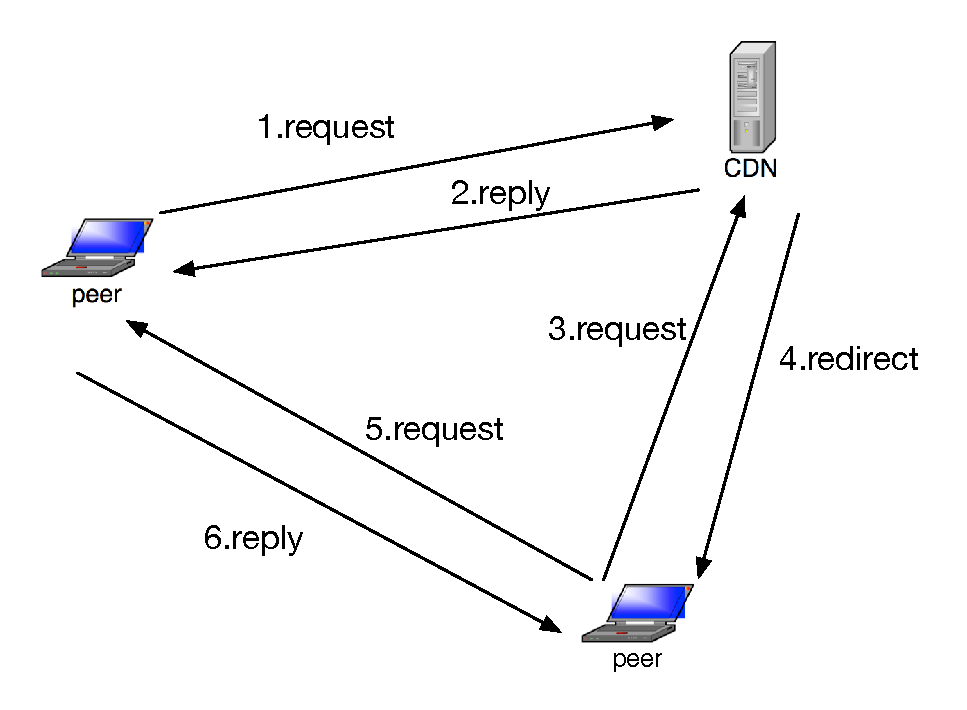
\includegraphics[scale=0.4]{graphs/p2p-system-description.eps}
\end{center}
\caption{Peer assisted CDN works as follows:
when a peer requests a video, it always goes to a CDN server (step 1). 
The CDN provides the videos to the peer (step 2). 
If there is another peer request same video, that request will go to CDN (step 3).  
A CDN will check its record to see if there is some peers cache that requested video.  
If there is some peers cache that requested video, a CDN will reply with redirect message that asking a peer to download requested video from other peer (step 4).
If there s no peers have requested video, a CDN will serve the video.   
A peer then can request the video to other peer and get the video (step 5 and step 6).
}
\label{fig:p2pcdninteractioninsimulator}
\end{figure} 



\section{System Description}\label{systemdescription}
%In our work, we use the Youtube VoD view model to aid our work that based from PROP. 
%The Youtube VoD view model will be used in our peer-caching strategy to exploit the video popularity while the caching strategy used in the CDN is out of scope for this project. 

\subsection{System Overview}\label{systemoverview}
The main components of the system are: (1) CDN and (2) peers which are self organized into a P2P overlay network.
%CDN itself consist of edge servers that deliver the videos and control plane servers that coordinate or control between the peers and record peers activities.
%The recording peers activities function is basically maintain a database of which videos are currently available on which peers as well as details about the connectivity of these peers.
%Peers appear in control plane database when uploading a video, a peer has a video to share, and a peer delete a video in its cache.
%In current peer-assisted CDN practice, the videos and their corresponding indices are decoupled.
%In other words, they are maintained by control plane servers.
Each peer in the system has two functionalities.
First, a peer is a client that requests a video. 
Second, a peer is a contributor or share the cached video with other peers in the system. 
Peers control the number and utilization of their connection based on current resources availability.
In fig.\ref{fig:p2pcdninteractioninsimulator}, we describe the process of a peer that requests a video which derived from PROP.
When a video is requested for the first time, the CDN is resposible to deliver the requested video.
When a CDN receives a query for a same video, a CDN will find suitable peers that currently have a copy of a requested video.
The CDN then returns information about these peers to the querying peer.
%In our system, the videos and their corresponding indices are decoupled because in current modern commercial peer-assisted CDN, CDN is responsible for recording each peer activities.  


\subsection{Peer caching strategy}\label{peercachingstrategy}
Since we only discuss peer-to-peer side, the caching strategy used in the CDN is out of scope for this project. 
For the peer replacement strategy, we introduce \textit{utility function} of a video as:
\begin{equation}
u = \frac{ (f(p) - f(p_{min})) (f(p_{max}) - f(p)) }{r^{\alpha + \beta}} + z(t)
\end{equation}
where the first term is the utility function from PROP and $z$ is the additional factor for CPPro. 
$p$ represents the popularity of the video, $p_{min}$ represents minimum popularity in the system, , $p_{max}$ represents maximum popularity in the system, and $r$ represents number of video replica.
Following \cite{1613869}, we can calculate $p$ as follows:
\begin{equation}
p = min \left(\frac{n_i^r}{t_i^r - t_a^i}  , \frac{1}{t_{cur} - t_i^r}\right)
\end{equation}
Where $n_i^r$ is number of requested video, $t_i^r$ is last time the video is requested, $t_a^i$ is the uploaded time of the video, and $t_{cur}$ is the current time.
To able to track the simulation, we use default value from PROP thus we refer the readers to \cite{1613869} for the details.

The utility function reflects the popularity of a video in the system that considering number of copy of its video or replica. 
$u$ value itself lies in interval $[0,2]$ Guo et al.,\cite{1613869}.
We choose video with the smallest utility value as the candidate to be replaced when a peer's cache is full.
Since we can determine before-peak phase, at-peak phase, and after-peak phase of video, we modified the original utility function from PROP above by adding a $z(t)$ factor as follows:

\begin{equation}
 z(t) = 
  \begin{cases}
   0.15 & \text{if phase estimation is before-peak} \\
   0.47 & \text{if phase estimation is at-peak} \\
   0.38 & \text{if phase estimation is after-peak}
  \end{cases}
\end{equation}\label{eq:zfactor}


$z(t)$ is proportion of view count in before-peak, at-peak, and after-peak to the total view count that we get from Youtube datasets.  
Because from transformed Youtube dataset we already have before-peak, at-peak, and after-peak phase for each video, we can also calculate how many view count in before-peak phase, at-peak phase, and after-peak phase.  
However at-peak happens only one week and its view count proportion to the total view count relatively small.
On the other side, we want to emphasize peer caching of a video during at-peak phase thus proportion of view count of at-peak phase to the total view count is count from one week before at-peak until one week after-peak.
Next we can count proportion of view count of before-peak and after-peak to the total view count.
The numbers of view count proportion for $z(t)$ is shown in eq.\ref{eq:zfactor}.

The value of $z(t)$ is assigned after we finish to determine a video popularity phase.  
For example: if we determine a video popularity phase is at-peak, then we assign $z(t)=0.47$.
%To able to track the simulation, we use default value from PROP thus we refer the readers to \cite{1613869}.
%$p$ represents popularity of the video, $p_{min}$ represents estimation of minimum popularity in P2P system, $p_{max}$ represents estimation of maximum popularity in P2P system, $r$ represents the number of replicas of the video in the system, and $f(p)$ is monotonic non-decreasing function.
%$\alpha$ and $\beta$ are the adjustment factor.
%The CDN can calculate $p_{min}$ and $p_{max}$ then propagate to the P2P system.
%To able to track the simulation, we use default value from PROP for $\alpha=\beta=1$ and $f(p)=log (p)$.
%We choose the video with the smallest $u$ value as the candidate to be replaced when a peer's cache capacity is full.
In PROP's utility function, the difference between very popular videos and unpopular video is very difficult to differentiate. 
For an unpopular video, $f(p)$ will be very close to $f(p_{min})$ thus $f(p) - f(p_{min})$ will be very close to $0$ then the utility function becomes very small.
For a very popular video, $f(p)$ will be very close to $f(p_{max})$, thus $f(p_{max}) - f(p)$ will be very close to $0$ and the  utility function becomes very small.  
Linear addition of $z(t)$ factor can help to differentiate the value of utility function.
%We summarize peer's decision for caching in pseudo code \ref{alg6}.

% \begin{algorithm}
% \caption{Peer decision}
% \label{alg6}
% \begin{algorithmic}[1]
% \REQUIRE a requested video popularity phase
% \STATE{calculate $p_{request}$ for a requested video}
% \IF{$phase$ $==$ $before$}
% \STATE{$z$ $\leftarrow$ $0.15$}
% \ELSIF{$phase$ $==$ $at$}
% \STATE{$z$ $\leftarrow$ $0.47$}
% \ELSE
% \STATE{$z$ $\leftarrow$ $0.38$}
% \ENDIF
% \STATE{get $p_{min}$ from CDN}
% \STATE{get $p_{max}$ from CDN}
% \STATE{get $r$ from CDN}
% \STATE{$u_{request}$ $\leftarrow$ $\frac{ (f(p_{request}) - f(p_{min})) (f(p_{max}) - f(p_{request})) }{r^{\alpha + \beta}} + z(t) $} \COMMENT{calculate u for a requested video}
% \FOR{every video inside peer's cache}\COMMENT{calculate $p$ and $u$ for every video inside peer's cache}
% \STATE{calculate $p$}
% \STATE{determine video popularity $phase$}
% \STATE{assign $z$ value}
% \STATE{get $r$ from CDN}
% \STATE{$u$ $\leftarrow$ $\frac{ (f(p) - f(p_{min})) (f(p_{max}) - f(p)) }{r^{\alpha + \beta}} + z(t)$ } \COMMENT{calculate u for a video inside peer's cache}
% \ENDFOR
% \STATE{$u_{min} \leftarrow min(u)$}
% \IF{$u_{request} > u_{min}$ }
% \IF{space not available}
% \STATE{delete video with $u_{min}$ inside peer's cache}
% \STATE{cache a requested video}
% \ELSE
% \STATE{cache a requested video}
% \ENDIF
% \ELSE
% \STATE{do not cache a requested video}
% \ENDIF
% \end{algorithmic}
% \end{algorithm}




\section{Evaluation}\label{evaluation}

In order to evaluate the proposed peer-caching strategy using our algoritmic designation of the poplarity phase of before-peak, at-peak, and after-peak information from Youtube VoD view model, we have to compare CPPro to the PROP model.
We evaluate three metrics, which are: (1) peer contribution to delivery contents during simulation,  access frequency of cache during simulation, and number of replicas. 
We define peer contribution as how many times a video is delivered by peer during simulation.
The peer contribution metric is related to the byte-hit-ratio. 
The byte-hit-ratio is defined as the total bytes of content served by peers normalized by the total bytes of video all peers and the CDN consume.
With more peer contributions, we will have higher byte-hit-ratio because peer can get content from other peers. 
However, because we only interested in peer performance, we compare peer contribution between PROP and CPPro.
Contribution ratio of peer (comparing to CDN contribution) is irrelevant in this case.
(2) Access frequency of cache reflects the storage utilization. 
More access means more peer storage utilization.  
(3) Number of replicas is also related to peer storage utilization.  
However, too many replicas will waste the storage resources.
To evaluate these metrics, we developed a peer-assisted CDN simulator. 


\subsection{Simulation Design}\label{simulationdesign}

This peer-assisted CDN is simulated using an event driven simulation implemented in Python. 
Peers request videos from a video catalog where the peer request as well as the videos in the catalog are generated using certain distributions.

%When a peer requests a video, it always goes to a CDN server (step 1). 
%The CDN provides the videos to the peer (step 2). 
%If there is another peer request same video, that request will go to CDN (step 3).  
%A CDN will check its record to see if there are some peers cache that requested video.  
%If there are some peers cache that requested video, a CDN will reply with redirect message that asking a peer to download requested video from other peer (step 4).
%If there are no peers have requested video, a CDN will serve the video.   
%A peer then can request the video to other peer and get the video (step 5 and step 6).
%From above description, we can see that deploying peer-assisted CDN can save some traffic since the clients which form P2P network can sharing the contents or videos.


\subsubsection{Video Catalog}\label{catalog}
Each video in tha catalog has the following properties: 
video-id,size,upload time, final view count, view count function parameters. 
View count parameters are the distribution parameters.
The final view count is the total number of views of a video at the end of simulation and it is generated using uniform distribution.
Upload time interval is a Poisson process with $\lambda=1$.
Video size is generated using a uniform distribution.
Because of the very weak relationship betwen video size and popularity \cite{abhari2010workload} and because our work focuses on the impact of the popularity aspect on the utility function rather than storage optimization we believe that the choice to assign a random uniform video size from the Youtube dataset does not have an effect to our results. 
The view rate progression from the upload time until the end of simulation time is modelled using a Beta distribution \cite{Borghol:2011:CMP:2039452.2039717}.
As Borghol et al.,\cite{Borghol:2011:CMP:2039452.2039717} showed that view rate of a video can be modelled using beta distribution we can calculate $\alpha$ and $\beta$ parameters.
Since we have view rate at peak, we can use Beta distribution mode formula to calculate $\alpha$ or $\beta$. In this case, we choose $\alpha$ random uniform between $1$ and $3$, thus $\beta$ parameter can be calculated using mode formula.
%The $\alpha$ and $\beta$ parameters are uniformly distributed. 


\subsubsection{Peer Request Generator}\label{peerrequest}
Peers request videos from the catalog using a Poisson process with $\lambda=1$ \cite{Zink:2009:CYN:1502814.1502987} for the inter-arrival time.
For the requested videos there are three scenarios namely A,B,and C.
Scenario A is where the video popularity in the peer-assisted CDN system follows the global popularity of the video.
Scenario B is where the video popularity in the peer-assisted CDN system lagging four weeks behind the global popularity of the video. 
We choose four weeks based on probability from time-to-peak distribution that half of videos are already reach peak within four weeks.
Scenario C is where the video popularity in the peer-assisted CDN system does not follow the global popularity of the video. 
We use Zipf distribution with rate$=0.9$ for this purpose \cite{6654887}.

% \subsubsection{Peer Request Generator}\label{peerrequest}
% There are three scenarios for peer request (named as scenario A, B, and C):
% In scenario A, a peer chooses a video that has popularity following Youtube.
% The objective of the first scenario, we want to see the peer requests effect to peer-assisted CDN when the request following Youtube popularity. 
% In scenario B, a peer chooses a video that has popularity following Youtube but we shift the request four weeks later.  
% The objective of the second scenario, we want to see the peer requests effect to peer-assisted CDN when the request from peers are shifted four weeks after popular in Youtube.
% %%why 4 weeks?
% In scenario C, a peer chooses a video that has popularity following zipf distribution with rate$=0.9$ \cite{6654887} thus a peer choose a video that its popularity does not follow Youtube popularity.
% The objective of the third scenario, we want to see the peer request effect to peer-assisted CDN when the requests from peers are totally different from Youtube's videos popularity.
% In all scenarios we assume peer interarrival time request a video following Poisson process with a mean rate $\lambda=1$ \cite{Zink:2009:CYN:1502814.1502987}.


%We assume that a peer choose a video based on a preference from view count and view rate that we can get from catalog generator.  
%Because peer requests are generate from catalog, the video request will follow global popularity video from YouTube


\subsubsection{Simulation Parameters}
The simulation parameters are follows:

\begin{itemize}
\item Length: $360$ days.
\item Video size: uniform random between $1$MB and $200$MB.
\item Peer storage capacity: $500$MB.
\item CDN storage capacity: $10000$MB.
\item Number of peers: $100000$.
\item Number of videos: $10000$.
\item Peer's caching strategy: CPPro, PROP.
\end{itemize}
Finally, we compare our results to PROP \cite{1613869} implementation.

%There are three scenarios in our simulations.
%First, peers choose a video that has a popularity following from Youtube data sets that we already explained in \ref{catalog}.
%Second, peers choose a video that has a popularity following from Youtube data sets and we shift the requests time four weeks.
%Third, peers choose a video that has a popularity following zipf distribution with rate$=0.9$ \cite{6654887}.
%We compare our results to original PROP \cite{1613869} implementation.



%%%%%%%%%%%%%%%%%%%%%%%%% FIGURE %%%%%%%%%%%%%%%%%%%%%%%%%%%%%%%%%%%
%%%contribution 
\begin{figure*}[!t]
\centering
\subfloat[Scenario A.\label{fig:contribu-normal}]{
\includegraphics[width=5.7cm]{graphs/new/repl/contributioncdnpeermodelsortedabs.eps}
}
\hfill
\subfloat[Scenario B.\label{fig:contribu-shift}]{
\includegraphics[width=5.7cm]{graphs/new/shift/contributioncdnpeermodelsortedabs.eps}
}
\hfill
\subfloat[Scenario C.\label{fig:contribu-zipf}]{
\includegraphics[width=5.7cm]{graphs/new/zipf/contributioncdnpeermodelsortedabs.eps}
}
\vspace{2mm}
\caption{Absolute peer contributions compared between CPPro and PROP ($y$-axis in log-scale and $y$-axis unit is times).}
\label{fig:peercontribution}
\end{figure*}
%%%%%%%%%%%%%%%%%%%%%%%%%% FIGURE %%%%%%%%%%%%%%%%%%%%%%%%%%%%%%%%%%%

%%%%%%%%%%%%%%%%%%%%%%%%% FIGURE %%%%%%%%%%%%%%%%%%%%%%%%%%%%%%%%%%%
%%%replica
\begin{figure*}[!t]
\centering
\subfloat[Scenario A.\label{fig:atd-normal}]{
\includegraphics[width=5.7cm]{graphs/new/repl/atd.eps}
}
\hfill
\subfloat[Scenario B.\label{fig:atd-shift}]{
\includegraphics[width=5.7cm]{graphs/new/shift/atd.eps}
}
\hfill
\subfloat[Scenario C.\label{fig:atd-zipf}]{
\includegraphics[width=5.7cm]{graphs/new/zipf/atd.eps}
}
\vspace{2mm}
\caption{Comparison of available replicas between model and prop when a peer requests a video ($y$-axis in log-scale).
In scenario C, we found many zero replica when a peer requests a video for CPPro. Because we use log-scale in this figure, the zero numbers can not be viewed}
\label{fig:replica}
\end{figure*}
%%%%%%%%%%%%%%%%%%%%%%%%%% FIGURE %%%%%%%%%%%%%%%%%%%%%%%%%%%%%%%%%%%


%%%%%%%%%%%%%%%%%%%%%%%%% FIGURE %%%%%%%%%%%%%%%%%%%%%%%%%%%%%%%%%%%
%%%replica
% \begin{figure*}[!t]
% \centering
% \subfloat[Percentage of cached and not-cached events for the first scenario.\label{fig:stacked1-normal}]{
% \includegraphics[width=5.7cm]{graphs/new/repl/stackedrepl1.eps}
% }
% \hfill
% \subfloat[Percentage of cached and not-cached events for the second scenario.\label{fig:stacked1-shift}]{
% \includegraphics[width=5.7cm]{graphs/new/shift/stackedshift1.eps}
% }
% \hfill
% \subfloat[Percentage of cached and not-cached events for the third scenario.\label{fig:stacked1-zipf}]{
% \includegraphics[width=5.7cm]{graphs/new/zipf/stackedzipf1.eps}
% }
% \vspace{2mm}
% \caption{Comparison of cached and not-cached events when a peer requests a video. For the model around $65\%$ events are not-cached event, while for PROP around $52\%$ events are cached event.}
% \label{fig:stacked1}
% \end{figure*}
%%%%%%%%%%%%%%%%%%%%%%%%%% FIGURE %%%%%%%%%%%%%%%%%%%%%%%%%%%%%%%%%%%


%%%%%%%%%%%%%%%%%%%%%%%%% FIGURE %%%%%%%%%%%%%%%%%%%%%%%%%%%%%%%%%%%
%%%replica
% \begin{figure*}[!t]
% \centering
% \subfloat[Video phase percentage in model for the first scenario and percentage of chaced and not-cached in PROP for the first scenario.\label{fig:stacked2-normal}]{
% \includegraphics[width=5.7cm]{graphs/new/repl/stacked-excel.eps}
% }
% \hfill
% \subfloat[Video phase percentage in model for the second scenario and percentage of chaced and not-cached in PROP for the second scenario.\label{fig:stacked2-shift}]{
% \includegraphics[width=5.7cm]{graphs/new/shift/stacked-excel.eps}
% }
% \hfill
% \subfloat[Video phase percentage in model for the third scenario and percentage of chaced and not-cached in PROP for the third scenario.\label{fig:stacked2-zipf}]{
% \includegraphics[width=5.7cm]{graphs/new/zipf/stacked-excel.eps}
% }
% \vspace{2mm}
% \caption{Video phase percentage in model for every scenario and percentage of cached and not-cached in PROP for every scenario.}
% \label{fig:stacked2}
% \end{figure*}
%%%%%%%%%%%%%%%%%%%%%%%%%% FIGURE %%%%%%%%%%%%%%%%%%%%%%%%%%%%%%%%%%%


%%%%%%%%%%%%%%%%%%%%%%%%% FIGURE %%%%%%%%%%%%%%%%%%%%%%%%%%%%%%%%%%%
%%%freq
\begin{figure*}[!t]
\centering
\subfloat[Frequency a video stays in peers for scenario A.\label{fig:freq-normal}]{
\includegraphics[width=5.7cm]{graphs/new/repl/freq.eps}
}
\hfill
\subfloat[Frequency a video stays in peers for scenario B.\label{fig:freq-shift}]{
\includegraphics[width=5.7cm]{graphs/new/shift/freq.eps}
}
\hfill
\subfloat[Frequency a video stays in peers for scenario C.\label{fig:freq-zipf}]{
\includegraphics[width=5.7cm]{graphs/new/zipf/freq.eps}
}
\vspace{2mm}
\caption{Frequency a video stays in peers compared between model and prop.}
\label{fig:freq}
\end{figure*}
%%%%%%%%%%%%%%%%%%%%%%%%%% FIGURE %%%%%%%%%%%%%%%%%%%%%%%%%%%%%%%%%%%

%%%%%%%%%%%%%%%%%%%%%%%%% FIGURE %%%%%%%%%%%%%%%%%%%%%%%%%%%%%%%%%%%
%%%duration
\begin{figure*}[!t]
\centering
\subfloat[Cache duration of a video in peers for scenario A.\label{fig:duration-normal}]{
\includegraphics[width=5.7cm]{graphs/new/repl/duration.eps}
}
\hfill
\subfloat[Cache duration of a video in peers for scenario B.\label{fig:duration-shift}]{
\includegraphics[width=5.7cm]{graphs/new/shift/duration.eps}
}
\hfill
\subfloat[Cache duration of a video in peers for scenario C.\label{fig:duration-zipf}]{
\includegraphics[width=5.7cm]{graphs/new/zipf/duration.eps}
}
\vspace{2mm}
\caption{Duration compared between model and prop.}
\label{fig:duration}
\end{figure*}
%%%%%%%%%%%%%%%%%%%%%%%%%% FIGURE %%%%%%%%%%%%%%%%%%%%%%%%%%%%%%%%%%%



\subsection{Result and Discussion}\label{resultanddiscussion}
%We define peer contribution as how many times a video is delivered by peer during simulation.

Figure~\ref{fig:peercontribution} shows the peer contribution in each scenario.
Peers are ranked by the number of videos served by each one.
They exhibit a similar pattern and only differ in the tails, where CPPro gives higher contributios, which are not significant to the total results as shown in fig.~\ref{fig:contribu-normal} and \ref{fig:contribu-shift}.
However, in the scenario C the peer contribution is almost identical in CPPro and PROP. 

The advantage of CPPro to PROP is shown in fig.~\ref{fig:replica} which show the number of replicas the requested videos at each request event.
We see that CPPro result in fewer replicas comparing to those of PROP.
Figure~\ref{fig:atd-zipf} that for scenario C,  CPPro has much fewer replicas than those of PROP.
It shows that many videos are not cached by CPPro.
That does not affect the peers contribution comparing to PROP.

%Since we only interested in peer performance, we compare peer contribution between PROP and CPPro.
%Contribution ratio of peer (comparing to CDN contribution) is irrelevant in this case.
%Figure \ref{fig:contribu-normal}, \ref{fig:contribu-shift}, and \ref{fig:contribu-zipf} show the absolute peer contribution to deliver videos comparing CPPro and PROP. 

%Figure \ref{fig:contribu-normal} and fig.\ref{fig:contribu-shift} exhibit the same pattern, with the peers giving more contribution in the tail.
%A peers can contribute mode because a video has longer duration than other videos in a peer's cache thus other peer's requests are served by the peer. 
%A video has longer duration than other videos in peer's cache because that a video has higher utility function than other videos for example a video that will enter the cache. 


% Figure \ref{fig:atd-normal}, \ref{fig:atd-shift}, and \ref{fig:atd-normal} show the number of  videos replicas available in system when a peer requests a video.
% As we can see from all figures, the model gives us lower number of replicas than PROP.
% The model gives lower number of replicas than PROP because when a peer requests a video, that peer is not cached the video.
% We can see the proportion of cached and not-cached event in table.\ref{tab:stacked1}. 
% We also present detail of the video phase breakdown in table.\ref{tab:stacked2}.
% In model, not-cached events take around $65\%$ from all events and majority of video phase is  after-peak for both cached events and not-cached events. 
% Because the majority of video phase is  after-peak for both cached events and not-cached events, 
% In PROP, cached events take around $52\%$ from all events for the first scenario and the second scenario, while for the third scenario is $67.7\%$.
% In model not-cached events are higher than PROP, means peers do not cached the videos thus we get lower replicas number than PROP.
%If we see eq.\ref{eq:dlms_3} and table.\ref{tab:stacked2}, we found that the majority of video phase is in after-peak for both cached events and not-cached events, then big probability that $z_{ms}$ and $z_{dl}$ are in the same phase which is after-peak phase.


% Denote $u_{dl}$ is the minimum utility function for a video inside the cache and $u_{ms}$ is utility function for a video that will enter the cache,  $p_{dl}$ is the popularity for a video inside the cache and $p_{ms}$ is the popularity for a video that will enter the cache.
% In order a requested video is cached by a peer, the utility function for $u_{dl}$ must be lower than the utility function for $u_{ms}$.

% \begin{align}\label{eq:dlms_1}
% u_{dl} < u_{ms}
% \end{align}

% \begin{multline}\label{eq:dlms_2}
% \frac{ (f(p_{dl}) - f(p_{min})) (f(p_{max}) - f(p_{dl})) }{r^{\alpha + \beta}_{dl}} + z_{dl} < \\
% \frac{ (f(p_{ms}) - f(p_{min})) (f(p_{max}) - f(p_{ms})) }{r^{\alpha + \beta}_{ms}} + z_{ms}
% %\end{equation}
% \end{multline}

% We assume that numbers of replicas are same, thus:
% \begin{multline}\label{eq:dlms_3}
% (f(p_{dl}) - f(p_{min})) (f(p_{max}) - f(p_{dl})) - \\ 
% (f(p_{ms}) - f(p_{min})) (f(p_{max}) - f(p_{ms})) < \\
% z_{ms} - z_{dl}
% \end{multline}

% Since $p_{min}$ and $p_{max}$ are same for $u_{dl}$ and $u_{ms}$, we can arrange the equation become:
% \begin{align}\label{eq:dlms_4}
% f(p_{ms}) - f(p_{dl}) > z_{dl} - z_{ms}
% \end{align}

%comparing with PROP, we can get: 
%\begin{align}\label{eq:dlms_5}
%f(p_{ms}) - f(p_{dl}) > 0 \\
%f(p_{ms}) - f(p_{dl}) > z_{dl} - z_{ms}
%\end{align}

% As we know from table.\ref{tab:stacked2} that the majority of a requested video is after-peak phase and a requested video phase that is  at-peak phase is very small portion, then we can see that $z_{dl} - z_{ms}$ term will be in negative term if $z_{dl}$ is  before-peak phase or $0$ if $z_{dl}$ is  after-peak phase. 
% If $z_{dl} - z_{ms}=0$ then it is same with PROP. 
% Since the not-cached events happen when a requested video phase is after-peak phase, we can get that $f(p_{ms}) - f(p_{dl}) < 0$.
% For the same situation and we compare to the PROP, the probability of $u_{ms}$ less than $u_{dl}$ in the model is higher than PROP. 
% Therefore, we can see in the model that the events when a peer does not cache a video are more often than PROP.

%It also means that $p_{ms}$ in after-peak phase less popular than $p_{dl}$.
%While comparing to PROP, the left term $f(p_{ms}) - f(p_{dl})$ will be equal to $0$ thus as result in CPPro a peer rejects the a requested video to be cached.

%If both videos are in the same phase (e.g before-peak, at-peak, or after-peak) then the difference between $p_{dl}$ and $p_{ms}$ is the only factor for utility function.
%However, if the videos are not in the same phase then the difference between $p_{dl}$ and $p_{ms}$ must always bigger than the difference between $z_{ms}$ and $z_{dl}$.
%There are two cases for the difference between $z_{ms}$ and $z_{dl}$.
%The first case is negative and the second case is positive.    
%The difference between $z_{ms}$ and $z_{dl}$ is positive when: 
%\begin{itemize}
%\item $z_{ms}$ is in at-peak period and $z_{dl}$ is in before-peak period.
%\item $z_{ms}$ is in at-peak period and $z_{dl}$ is in after-peak period.
%\item $z_{ms}$ is in after-peak period and $z_{dl}$ is in before-peak period.
%\end{itemize}
%When the difference between $z_{ms}$ and $z_{dl}$ is negative, the difference between $p_{dl}$ and $p_{ms}$ is the only factor for utility function.

\begin{table*}[!t]
%% increase table row spacing, adjust to taste
%\renewcommand{\arraystretch}{1.3}
% if using array.sty, it might be a good idea to tweak the value of
% \extrarowheight as needed to properly center the text within the cells
\caption{Percentage of Cached events and Not-Cached events in CPPro and PROP}
\label{tab:stacked1}
\centering
%% Some packages, such as MDW tools, offer better commands for making tables
%% than the plain LaTeX2e tabular which is used here.
\begin{tabular}{|l|l|c|c|c|c|}
\hline
Scenario & Type & Cached (times)& Not-Cached (times) & Cached (PetaByte) & Not-Cached (PetaByte)\\
\hline
A & CPPro & $33.5\%$ & $66.5\%$ & $2422$ & $4808$ \\
\hline
 & PROP & $52\%$ & $48\%$ & $2416$ & $2230$\\
\hline

B & CPPro & $34.8\%$ & $65.2\%$ & $2423$ & $4540$\\
\hline
 & PROP & $52.6\%$ & $47.4\%$  &  $2415$  &  $2176$ \\
\hline

C & CPPro & $32.4\%$ & $67.6\%$  & $2435.5$ & $5079.5$ \\
\hline
 & PROP & $67.7\%$ & $32.3\%$ &  $2435.3$ & $1161.9$ \\
\hline
\end{tabular}
\end{table*}


\begin{table*}[!t]
%% increase table row spacing, adjust to taste
%\renewcommand{\arraystretch}{1.3}
% if using array.sty, it might be a good idea to tweak the value of
% \extrarowheight as needed to properly center the text within the cells
\caption{Percentage of Video Phase for Model in cached and not-cached events}
\label{tab:stacked2}
\centering
%% Some packages, such as MDW tools, offer better commands for making tables
%% than the plain LaTeX2e tabular which is used here.
\begin{tabular}{|l|l|c|c|c|}
\hline
Scenario & Type/Events & Before-Peak & At-Peak  & After-Peak \\
\hline
A & Model-Cached & $8.2\%$ & $1.2\%$ & $24.1\%$  \\
\hline
 & Model-Not-Cached & $11.2\%$ & $0.8\%$ & $54.5\%$ \\
 \hline

B & Model-Cached & $6.2\%$ & $1.2\%$ & $29.8\%$ \\
\hline
 & Model-Not-Cached & $5.2\%$ & $0.8\%$ & $56.8\%$ \\
\hline

C & Model-Cached & $8.0\%$ & $1.8\%$ & $22.7\%$ \\
\hline
 & Model-Not-Cached & $15.1\%$ & $0.8\%$ & $51.6\%$ \\
\hline
\end{tabular}
\end{table*}

Figure \ref{fig:freq-normal}, \ref{fig:freq-shift}, and \ref{fig:freq-zipf} show the frequency of a video stay in peers compared between model and PROP.
As all figure show the model has higher frequency than PROP to stay in peers except for the beginning rank of data where the model has same frequency with prop in first and second scenario. 
In the third scenario, in the beginning rank of data the model has lower frequency than PROP, then around rank 1000 the model has higher frequency than prop until the end of data. 
The frequency a video stay in a video can also be viewed in fig \ref{fig:duration-normal},  \ref{fig:duration-shift}, and \ref{fig:duration-zipf}, where in the model some videos have longer cache duration than PROP, while others have shorter cache duration than PROP.  
Thus, we can see the relationship between cache duration and frequency a video stays in peers. 

\section{Conclusion and Future Work}\label{conclusion}
This paper presents a scheme for peer-to-peer network can help CDN to deliver the content over the Internet. 
We show that by introducing $z$ factor to utility function we can maintain same peer contribution while reducing number of replicas.
We found that there are no much different between the first scenario, the second scenario and the third scenario in peer contribution to deliver a video. 
We found that in the all scenarios, the model gives lower replicas than PROP. 
This is because in the model, we found that not-cached events are higher than cached events, more specifically, the probability of utility function a requested video in model is lower than PROP.
Therefore, in the model the numbers of available replicas are lower than PROP. 
We also did the significance test to the number of replicas using the Kolmogorov-Smirnov statistic on two samples and we find that for all scenarios the $p$-values are less than $1$\% thus the results are significant. 

Some areas of improvement that we have identified for future are:
The energy trade off this peer-assisted CDN architecture in order to know how much energy saving by ISP and how much increase of energy at users home gateway side in this architecture since we have higher peer contribution.   
More numerical experiments for other zipf shape parameters. 


% use section* for acknowledgement
\section*{Acknowledgment}
The authors would like to thank Internet research laboratory member at Keio University and anonymous reviewers.





% trigger a \newpage just before the given reference
% number - used to balance the columns on the last page
% adjust value as needed - may need to be readjusted if
% the document is modified later
%\IEEEtriggeratref{8}
% The "triggered" command can be changed if desired:
%\IEEEtriggercmd{\enlargethispage{-5in}}

% references section

% can use a bibliography generated by BibTeX as a .bbl file
% BibTeX documentation can be easily obtained at:
% http://www.ctan.org/tex-archive/biblio/bibtex/contrib/doc/
% The IEEEtran BibTeX style support page is at:
% http://www.michaelshell.org/tex/ieeetran/bibtex/
%\bibliographystyle{IEEEtran}
% argument is your BibTeX string definitions and bibliography database(s)
%\bibliography{IEEEabrv,../bib/paper}
%
% <OR> manually copy in the resultant .bbl file
% set second argument of \begin to the number of references
% (used to reserve space for the reference number labels box)
\bibliographystyle{IEEEtran}
\bibliography{manu}

% that's all folks
\end{document}


